% !TEX root = ../../main.tex
%======================================================================
\section{Learning Problem}
\label{sec:learning}
%======================================================================

In this section, we examine the regulatory setting under incomplete information, where the underlying joint market distribution $(X, Y, \{N_j\})$ is unknown to the regulator. We formulate the regulator's search for optimal enforcement tolerance $\varepsilon^*$ as an online continuum-armed bandit problem.\index{Online regulatory learning|textbf} We apply the well-established framework of Gaussian Process Thompson Sampling (GP-TS)~\cite{chowdhury2017kernelized} to analyze learning performance in our strategic IPO regulation setting.

At each round $t = 1, \dots, T$, the regulator selects an enforcement tolerance $\varepsilon_t \in [0, \varepsilon_{\max}]$ and subsequently observes the realized social welfare $W_t = \mathcal{W}(\varepsilon_t) + \xi_t$, where $\xi_t = W_t - \mathcal{W}(\varepsilon_t)$ represents zero-mean observation noise arising from market realization randomness.

Under Assumption~\ref{ass:regularity}, the expected social welfare function $\mathcal{W}(\varepsilon)$ is $C^{\infty}$ over the compact domain $[0, \varepsilon_{\max}]$. Because $C^{\infty}([0, \varepsilon_{\max}])$ is densely embedded in the Sobolev space $H^3([0, \varepsilon_{\max}])$, which is norm-equivalent to the Reproducing Kernel Hilbert Space (RKHS) $\mathcal{H}_k$ of the Mat\'ern-$5/2$ kernel (for comprehensive background on Mat\'ern kernels and RKHS properties, see, e.g., \cite{rasmussen2006gaussian, chowdhury2017kernelized}):
\begin{equation}
\label{eq:matern}
\begin{aligned}
k_{5/2}(\varepsilon, \varepsilon')
&= \sigma_0^2 \biggl( 1 + \frac{\sqrt{5}\,|\varepsilon-\varepsilon'|}{l} + \frac{5(\varepsilon-\varepsilon')^2}{3l^2} \biggr) \\
&\quad \times \exp\biggl( -\frac{\sqrt{5}\,|\varepsilon-\varepsilon'|}{l} \biggr),
\end{aligned}
\end{equation}
it follows directly that $\mathcal{W} \in \mathcal{H}_k$ with a bounded RKHS norm $\|\mathcal{W}\|_{\mathcal{H}_k} \le B < \infty$. Here $\sigma_0^2 > 0$ is the signal variance and $l > 0$ is the characteristic length-scale parameter (for detailed information about Matérn kernels and RKHS refer \cite{chowdhury2017kernelized}).

The regulator employs GP-TS (Algorithm~\ref{alg:gpts}) to adaptively select $\varepsilon_t$. By placing a GP prior $\mathcal{GP}(0, k_{5/2})$ over $\mathcal{W}$, the regulator maintains posterior mean $\mu_{t-1}(\cdot)$ and covariance $k_{t-1}(\cdot,\cdot)$ updated via standard Gaussian process regression equations over past history $\mathcal{H}_{t-1} = \{(\varepsilon_\tau, W_\tau)\}_{\tau=1}^{t-1}$:
\begin{equation}
\label{eq:gp_update}
\begin{aligned}
\mu_{t-1}(\varepsilon) &= k_{t-1}(\varepsilon)^\top (K_{t-1} + \sigma^2 I)^{-1} \mathbf{W}_{t-1}, \\
k_{t-1}(\varepsilon, \varepsilon') &= k_{5/2}(\varepsilon, \varepsilon') - k_{t-1}(\varepsilon)^\top (K_{t-1} + \sigma^2 I)^{-1} k_{t-1}(\varepsilon'),
\end{aligned}
\end{equation}
where $k_{t-1}(\varepsilon) = [k_{5/2}(\varepsilon_1, \varepsilon), \dots, k_{5/2}(\varepsilon_{t-1}, \varepsilon)]^\top$, $K_{t-1}$ is the $(t-1) \times (t-1)$ kernel matrix with entries $[K_{t-1}]_{ij} = k_{5/2}(\varepsilon_i, \varepsilon_j)$, and $\mathbf{W}_{t-1} = [W_1, \dots, W_{t-1}]^\top$.

\begin{algorithm}[t]\index{Gaussian Process Thompson Sampling!for IPO regulation|textbf}
\caption{Gaussian Process Thompson Sampling (GP-TS) for IPO Regulation}
\label{alg:gpts}
\begin{algorithmic}[1]
\State \textbf{Input:} Mat\'ern-$5/2$ kernel $k_{5/2}(\cdot,\cdot)$, GP prior $\mathcal{GP}(0, k_{5/2})$, domain $[0, \varepsilon_{\max}]$, horizon $T$, noise variance $\sigma^2$, confidence $\delta \in (0,1)$.
\For{$t = 1, 2, \dots, T$}
  \State Set inflation factor $v_t = B + R\sqrt{2(\gamma_{t-1} + 1 + \log(2/\delta))}$ \citep{chowdhury2017kernelized}.
  \State Compute GP posterior mean $\mu_{t-1}(\varepsilon)$ and covariance $k_{t-1}(\varepsilon,\varepsilon')$ using~\eqref{eq:gp_update} based on history $\mathcal{H}_{t-1}$.
  \State Sample function candidate $\widetilde{\mathcal{W}}_t \sim \mathcal{GP}(\mu_{t-1},\, v_t^2 k_{t-1})$.
  \State Select regulatory enforcement tolerance $\varepsilon_t \in \arg\max_{\varepsilon \in \mathcal{D}_t} \widetilde{\mathcal{W}}_t(\varepsilon)$ over round-$t$ net $\mathcal{D}_t \subset [0, \varepsilon_{\max}]$.
  \State Apply $\varepsilon_t$ to the market and observe realized social welfare $W_t$.
  \State Update interaction history $\mathcal{H}_t = \mathcal{H}_{t-1} \cup \{(\varepsilon_t, W_t)\}$ and update posterior parameters.
\EndFor
\end{algorithmic}
\end{algorithm}

Applying the established regret analysis of GP-TS for kernelized continuum-armed bandits~\cite{chowdhury2017kernelized} directly specializes the general sublinear regret guarantee to our strategic IPO regulation problem.

\begin{theorem}[Regret Guarantee for IPO enforcement tolerance]
\label{thm:regret}
Under Assumption~\ref{ass:regularity}, if the regulator employs GP-TS (Algorithm~\ref{alg:gpts}) with the Mat\'ern-$5/2$ kernel $k_{5/2}$, the cumulative regret $R_T = \sum_{t=1}^T \bigl(\mathcal{W}(\varepsilon^*) - \mathcal{W}(\varepsilon_t)\bigr)$ is bounded with probability at least $1-\delta$ by
\begin{equation}
\label{eq:rt_bound}
R_T = \widetilde{\mathcal{O}}\!\left(T^{2/3}\right).
\end{equation}
\end{theorem}

\begin{proof} The proof is given in Section~\ref{sec:proofs_ch5} (Proof~\ref{proof:thm_regret}).
\end{proof}

To empirically validate the learning performance of the GP-TS algorithm in regulatory enforcement design, we simulate the continuous bandit problem across independent trials.\coderef{subsec:code_ipo_learning} We consider an underlying market environment with $k=2$ investor subpopulations of equal size ($N_1 = N_2 = 50$, $\mathcal{N} = 100$, $\eta = 1$), baseline feature $X \sim U[-1/3, 1/3]$, and linear valuation profiles $V_1(z) = 1+3z$ and $V_2(z) = 1-3z$. The firm's true valuation $Y(X)$ takes value in $\{V_1(X), V_2(X)\}$ according to probabilities $\gamma_1(X)$ and $\gamma_2(X)$, inducing observation noise in realized social welfare $W_t$; we evaluate learning performance under two noise conditions: low noise ($\sigma = 0.05$) and high noise ($\sigma = 0.25$). At each round $t$, after selecting enforcement strictness $\varepsilon_t \in [0, 1.2]$, the regulator observes realized social welfare $W_t$.

The cumulative regret trajectories ($R_T$) displayed in Figure~\ref{fig:learning} exhibit sublinear growth bounded by the theoretical $\widetilde{\mathcal{O}}(T^{2/3})$ rate established in Theorem~\ref{thm:regret} across both noise levels (shaded bands denote $\pm 1$ standard error across $40$ independent trials).

\begin{figure}[t]
\centering
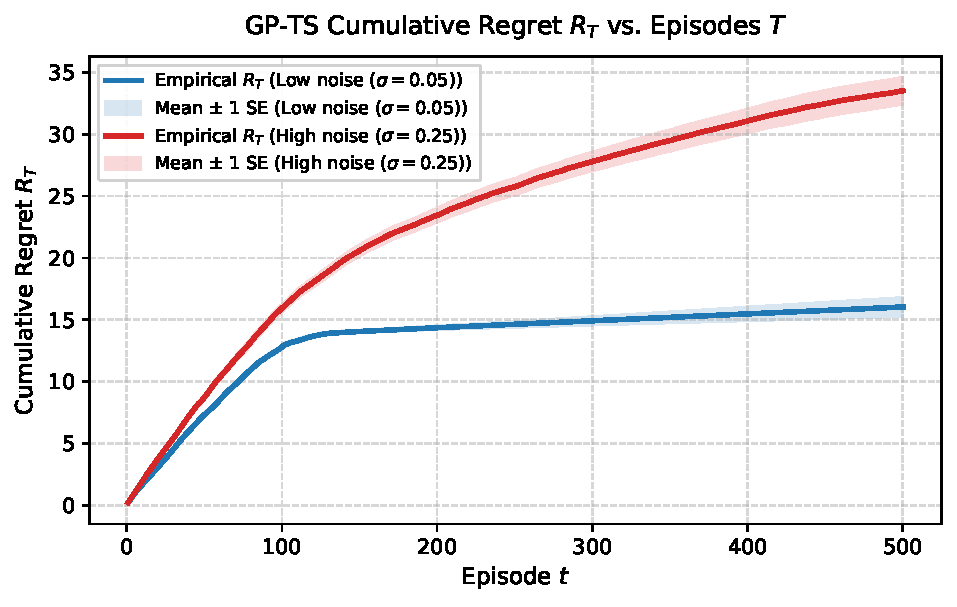
\includegraphics[width=0.72\columnwidth]{figures/learning_results.pdf}
\caption{Cumulative regret $R_T$ of GP-TS online regulatory learning under low ($\sigma=0.05$) and high ($\sigma=0.25$) noise (solid curves show mean cumulative regret, shaded bands indicate $\pm 1$ standard error across $40$ trials).}
\label{fig:learning}
\end{figure}

